\section{结果}
\label{sec:results}
\subsection{审计识别出一个缺少源支持的目标叶类别}
\label{sec:gap_result}
图\ref{fig:coverage}概括操作性覆盖记录。LoveDA 为六个叶类别提供精确的操作性支持，但不包含草本植被。FLAIR 原始 ID 10 提供所声明的辅助草本标签，其余 FLAIR 标签在 B1 中均被忽略。在冻结映射下，OpenEarthMap \texttt{rangeland} 和 Semantic Drone \texttt{grass} 被声明为同一非耕地草本概念所对应的目标类别。数据总体和源角色见表\ref{tab:datasets}。
\begin{figure}[H]
\centering
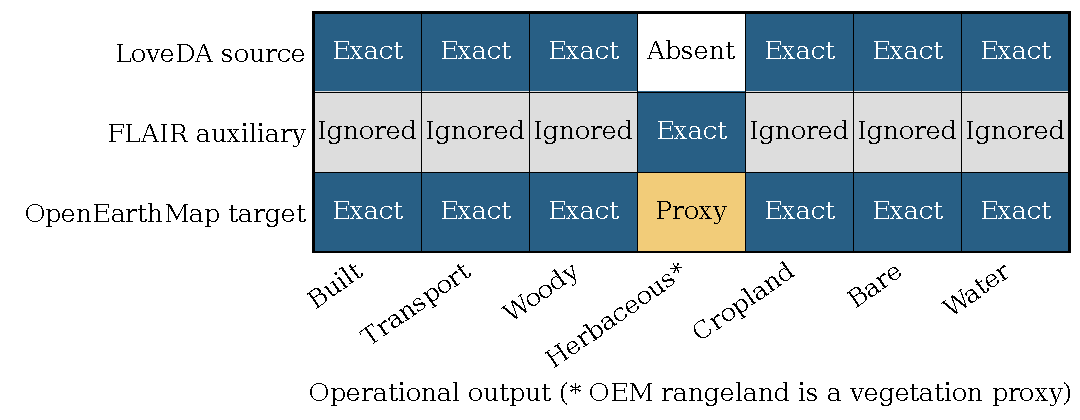
\includegraphics[width=0.92\textwidth]{fig1_coverage_20261015.pdf}
\caption{主要源混合与 OpenEarthMap 目标的操作性覆盖。Exact 表示原始标签在固定映射下被分配到相应公共叶类别，不表示普遍语义等价。LoveDA 没有被纳入草本输出的源标签。B1 保留 FLAIR 原始 ID 10，忽略其余标签。OEM 的 Proxy 单元反映 rangeland 包括灌木的较宽定义（英文补充材料 S2）。Semantic Drone 单独按草地对全部其他像素评估（第\ref{sec:semanticdrone_result}节）。}
\label{fig:coverage}
\end{figure}

\subsection{加入 FLAIR 辅助源能够恢复 OpenEarthMap rangeland}
\label{sec:oem_result}
主要对比中最大的变化集中在经审计缺失的叶类别。种子19、37、73的三个固定检查点上，B0 rangeland IoU 分别为$1.6\times10^{-7}$、0、0，B1 则为0.3124、0.3187、0.3041。在排除 Paris 的74城总体上，配对平均差值为+0.3118，95\%评估单位 bootstrap 区间为[+0.2821, +0.3399]（表\ref{tab:oem-seeds}、图\ref{fig:oem-primary}）。该区间对所声明城市单位重采样，并以已完成检查点为条件。
\begin{figure}[H]
\centering
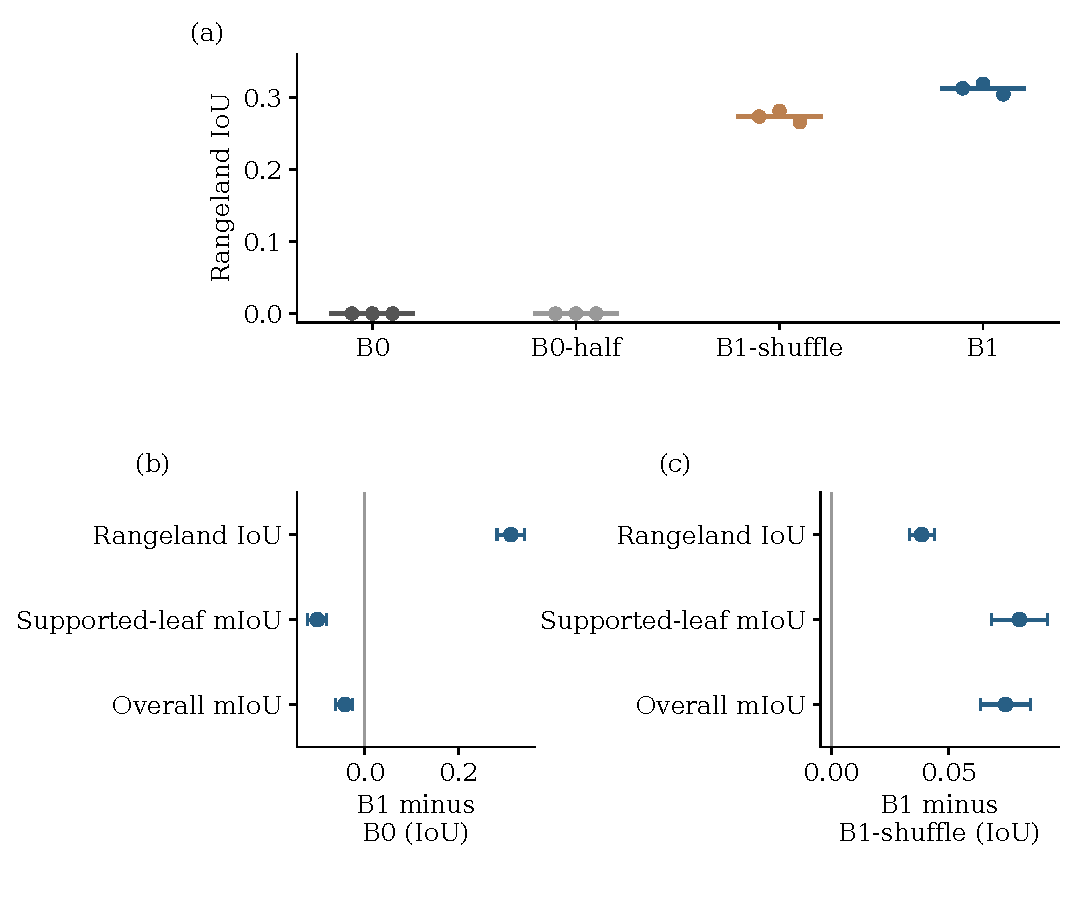
\includegraphics[width=0.92\textwidth]{fig2_oem_results_20261015.pdf}
\caption{排除 Paris 后74城总体上的 OpenEarthMap 结果。（a）种子19、37、73的 rangeland IoU，水平短线表示均值，横向偏移用于区分检查点。（b）B1 减 B0。（c）B1 减已记录的 B1-shuffle 配置。（b）和（c）采用不同坐标范围，显示2,000次配对城市重采样得到的95\%区间，以三个已完成检查点为条件。支持类别 mIoU 对六个 LoveDA 支持类别平均。完整原始 shuffle 排程未找回，因此（c）仅是基于配置的敏感性，而非完整重验证的配对机制。}
\label{fig:oem-primary}
\end{figure}
仅减少 LoveDA 暴露量不能重复目标叶类别的恢复。相对 B0，B0-half 总体 mIoU 降低0.0069；在匹配 LoveDA 暴露后，B1 的 rangeland 收益仍为+0.3118（表\ref{tab:oem-controls}）。重复裁块完整性检查在所报告精度下为零，见附录表\ref{tab:batch_integrity}；它检查更新实现，而不是一般性的批大小效应。

\subsection{对已记录配对配置的敏感性}
\label{sec:pairing_result}
历史 B1-shuffle 配置要求采用相同的 FLAIR 影像排程和掩膜密度多重集，但使用非原生配对掩膜。完整原始排程未找回，因此这些约束无法独立重新验证。该配置仍能恢复 rangeland，三个种子的 IoU 分别为0.2732、0.2812、0.2653。相对 B0 的平均差值为0.2732，而 B1--B0 为0.3118。因此，0.2732/0.3118 = 87.6\%的观察恢复量保留在该错配排程中；原生 B1 配置再提高+0.0385（12.4\%；95\%评估单位 bootstrap 区间[+0.0333, +0.0439]），三个种子的配对差值均为正。同一对比中，总体 mIoU 提高+0.0741，六个 LoveDA 支持类别 mIoU 提高+0.0801（表\ref{tab:oem-controls}）。这一算术划分仅描述指定排程，不分离辅助影像内容和标签支持。由于主要原始排程无法独立重新验证，本文将其作为基于配置的敏感性，而非完整验证的配对机制。
\begin{table}[H]
\centering
\caption{排除 Paris 后74城 OpenEarthMap 各固定检查点指标。数值显示四位小数；种子19的 B0 rangeland IoU 为$1.6\times10^{-7}$，种子37和73为零。B0 与 B1 的支持类别 mIoU 范围分别为0.4359--0.4468与0.3309--0.3473。支持类别 mIoU 对六个具有 LoveDA 精确操作性支持的类别平均，与总体 mIoU 并列报告，而非另一总体性能估计。城市 bootstrap 差值根据未舍入检查点指标计算，仅展示时舍入（表\ref{tab:oem-controls}）。}
\label{tab:oem-seeds}
\small
\renewcommand{\arraystretch}{1.12}
\setlength{\tabcolsep}{4pt}
\begin{tabular*}{\linewidth}{@{\extracolsep{\fill}}lrrrr@{}}
\toprule
分支 & 种子 & 总体 mIoU & Rangeland IoU & 支持类 mIoU \\
\midrule
B0 & 19 & 0.3830 & 0.0000 & 0.4468 \\
B0 & 37 & 0.3802 & 0.0000 & 0.4436 \\
B0 & 73 & 0.3736 & 0.0000 & 0.4359 \\
B0-half & 19 & 0.3652 & 0.0000 & 0.4261 \\
B0-half & 37 & 0.3825 & 0.0000 & 0.4462 \\
B0-half & 73 & 0.3683 & 0.0000 & 0.4296 \\
B1-shuffle & 19 & 0.2710 & 0.2732 & 0.2707 \\
B1-shuffle & 37 & 0.2564 & 0.2812 & 0.2523 \\
B1-shuffle & 73 & 0.2604 & 0.2653 & 0.2596 \\
B1 & 19 & 0.3400 & 0.3124 & 0.3446 \\
B1 & 37 & 0.3292 & 0.3187 & 0.3309 \\
B1 & 73 & 0.3411 & 0.3041 & 0.3473 \\
\bottomrule
\end{tabular*}
\end{table}

\begin{table}[H]
\centering
\caption{排除 Paris 后74城 OpenEarthMap 固定预算和错配配对控制差值。区间为以已完成固定检查点为条件的配对城市 bootstrap 区间。差值使用未舍入检查点指标计算，仅展示时舍入。重复裁块完整性检查见附录表\ref{tab:batch_integrity}。}
\label{tab:oem-controls}
\small
\renewcommand{\arraystretch}{1.12}
\setlength{\tabcolsep}{4pt}
\begin{tabular*}{\linewidth}{@{\extracolsep{\fill}}llrrr@{}}
\toprule
对比 & 指标 & 估计 & 95\%下界 & 95\%上界 \\
\midrule
B0-half $-$ B0 & 总体 mIoU & $-0.0069$ & $-0.0100$ & $-0.0038$ \\
B1 $-$ B0 & 总体 mIoU & $-0.0422$ & $-0.0613$ & $-0.0252$ \\
B1 $-$ B0 & rangeland IoU & $+0.3118$ & $+0.2821$ & $+0.3399$ \\
B1 $-$ B0-half & 总体 mIoU & $-0.0352$ & $-0.0538$ & $-0.0182$ \\
B1 $-$ B0-half & rangeland IoU & $+0.3118$ & $+0.2821$ & $+0.3399$ \\
B1 $-$ B0 & 支持类 mIoU & $-0.1011$ & $-0.1213$ & $-0.0821$ \\
B1 $-$ B0-half & 支持类 mIoU & $-0.0931$ & $-0.1128$ & $-0.0741$ \\
B1 $-$ B1-shuffle & 总体 mIoU & $+0.0741$ & $+0.0634$ & $+0.0848$ \\
B1 $-$ B1-shuffle & 支持类 mIoU & $+0.0801$ & $+0.0682$ & $+0.0921$ \\
B1 $-$ B1-shuffle & rangeland IoU & $+0.0385$ & $+0.0333$ & $+0.0439$ \\
\bottomrule
\end{tabular*}
\end{table}


\subsection{恢复伴随源支持类别性能损失}
\label{sec:tradeoff_result}
目标叶类别的收益没有改善完整运行表现。B1 平均 mIoU 为0.3368，B0 为0.3789；对六个具有 LoveDA 精确操作性支持的类别，mIoU 变化为-0.1011（95\%评估单位 bootstrap 区间[-0.1213, -0.0821]）。这两个指标回答不同问题：总体 mIoU 包含恢复后的 rangeland，支持类别指标则排除该类，单独报告 LoveDA 原有类别保持。两者的数值差异不是相互竞争的效应量估计。B0 各种子支持类别 mIoU 为0.4359至0.4468，B1 为0.3309至0.3473（表\ref{tab:oem-seeds}）；推断仍基于城市单位 bootstrap，而非三个种子的显著性检验。匹配 LoveDA 暴露后，B1--B0-half 的支持类别差值为-0.0931（表\ref{tab:oem-controls}）。图\ref{fig:oem-tradeoff}展示逐类模式：rangeland 恢复，但观察到的支持类别最大下降出现在耕地。完整、未调整的描述性区间见附录表\ref{tab:all_leaf_contrasts}。
\begin{figure}[H]
\centering
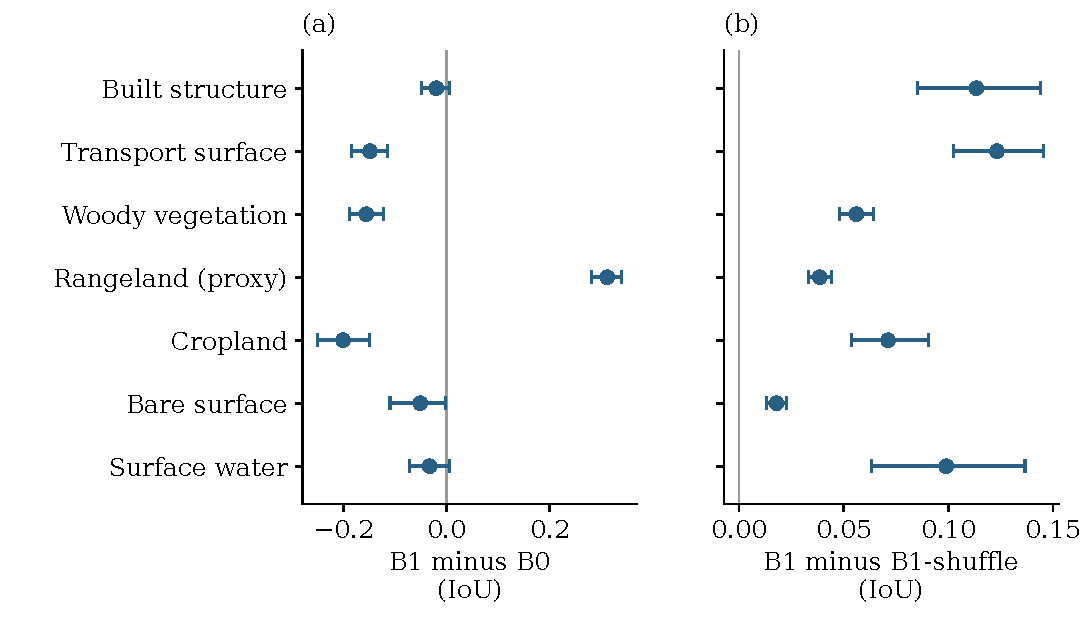
\includegraphics[width=0.92\textwidth]{fig3_leaf_contrasts_20261015.pdf}
\caption{排除 Paris 后74城总体上的 OpenEarthMap 逐类差值。（a）B1 减 B0；（b）B1 减已记录的 B1-shuffle。两个面板采用相同的七个类别行，报告2,000次配对城市重采样的95\%描述性区间，以检查点19、37、73为条件。（b）为基于配置的敏感性：完整原始 shuffle 排程未找回，无法独立重验证配对与暴露约束。两个面板横轴尺度不同。}
\label{fig:oem-tradeoff}
\end{figure}

\subsection{历史原生 U-Net 对比重复了相同方向}
\label{sec:unet_result}
在三个历史原生 U-Net 检查点上，U-B0 与 U-B0-half 的 rangeland IoU 均为零。U-B1 分别为0.2957、0.2767、0.2762，平均0.2828，样本标准差0.0111。U-B1--U-B0 的差值为+0.2828（以检查点为条件的95\%配对城市区间[+0.2512, +0.3133]）。支持类别 mIoU 从0.2329变为0.1025，差值-0.1304（区间[-0.1529, -0.1075]）；相对 U-B0-half 的差值为-0.1182（区间[-0.1390, -0.0965]）。与两个原生基线比较时，每个匹配种子均表现为 rangeland 恢复为正、支持类别 mIoU 下降（表\ref{tab:unet-native}）。

因此，历史评估记录在共同目标上的第二种记录架构中显示了恢复与保持损失并存。它们没有提供独立目标总体、纯标签因果实验或 CLIP--U-Net 优越性比较。原始检查点、空间参考与历史代码的来源限制仍如第\ref{sec:unet_protocol}节所述。U-Net shuffle 结果不参与该结论。
\begin{table}[H]
\centering
\caption{同一排除 Paris 后74城 OpenEarthMap 目标（2,638张栅格）上的历史原生 U-Net 对比。均值与样本标准差汇总三个已记录种子检查点，标准差为描述性统计。差值使用2,000次配对城市抽样，95\%区间以固定记录检查点为条件，不代表训练种子不确定性。支持类别 mIoU 对六个 LoveDA 支持类别平均。U-B0-half 匹配 U-B1 的 LoveDA 暴露量。未重放原始检查点和空间参考字节；这是家族内部的历史记录对比。}
\label{tab:unet-native}
\small
\setlength{\tabcolsep}{3pt}
\begin{tabular*}{\linewidth}{@{\extracolsep{\fill}}lrrr@{}}
\toprule
分支 & Rangeland IoU & 支持类 mIoU & 总体 mIoU \\
\midrule
U-B0 & $0.0000 \pm 0.0000$ & $0.2329 \pm 0.0158$ & $0.1996 \pm 0.0136$ \\
U-B0-half & $0.0000 \pm 0.0000$ & $0.2207 \pm 0.0261$ & $0.1892 \pm 0.0223$ \\
U-B1 & $0.2828 \pm 0.0111$ & $0.1025 \pm 0.0209$ & $0.1283 \pm 0.0190$ \\
\bottomrule
\end{tabular*}
\par\medskip
\begin{tabular*}{\linewidth}{@{\extracolsep{\fill}}lrrr@{}}
\toprule
对比与指标 & 估计 & 95\%下界 & 95\%上界 \\
\midrule
U-B1 $-$ U-B0 / rangeland & $+0.2828$ & $+0.2512$ & $+0.3133$ \\
U-B1 $-$ U-B0 / 支持类 & $-0.1304$ & $-0.1529$ & $-0.1075$ \\
U-B1 $-$ U-B0-half / rangeland & $+0.2828$ & $+0.2512$ & $+0.3133$ \\
U-B1 $-$ U-B0-half / 支持类 & $-0.1182$ & $-0.1390$ & $-0.0965$ \\
\bottomrule
\end{tabular*}
\end{table}


\subsection{Semantic Drone 上的第二目标评估}
\label{sec:semanticdrone_result}
在主要400张栅格评估中，冻结 E0 的 grass IoU 为0.0224，三个仅用 LoveDA 的 B0 检查点均为0.0000。三个 B1 检查点分别为0.2282、0.2305、0.2228（均值0.2272，样本标准差0.0040）。描述性的 B1--B0 平均差值为+0.2272（英文补充材料 S9 和 S11）。本稿不主张具有三个检查点的栅格重采样区间。E0 到 B0 的下降是检查点诊断，与仅用 LoveDA 校准抑制冻结探针已有的有限 grass 分数相一致，但不能识别具体机制。这是主要源混合在第二目标上的评估，并非模型层面的独立复现，因为它复用了探针、提示词和训练预算。历史记录指明目标清单与源归档哈希，但本文未建立具有独立时间戳的推理前来源证据。

\subsection{第二种源混合呈现相同的恢复—损失方向}
\label{sec:second_mixture_result}
源角色反向配置从另一个经审计缺口出发：Semantic Drone 没有精确的操作性耕地标签，而 LoveDA agriculture 和 OpenEarthMap \texttt{agriculture\_land} 提供所声明的耕地关系。在冻结的72城 OpenEarthMap 总体上，SD-B0 与暴露匹配的 SD-B0-half 在每个种子上的耕地 IoU 均为零。SD-B1 为0.1627、0.1642、0.1627，平均配对 SD-B1--SD-B0 差值为+0.1632（95\%评估单位 bootstrap 区间[+0.1262, +0.2049]；表\ref{tab:second-mixture}）。

恢复同样伴随固定预算下的代价。在三个具有 Semantic Drone 精确操作性支持的叶类别上，SD-B1 相对 SD-B0 的基础源 mIoU 变化为-0.1686（95\%评估单位 bootstrap 区间[-0.1903, -0.1464]），相对暴露匹配 SD-B0-half 为-0.1337（区间[-0.1534, -0.1151]）。原计划的辅助掩膜 shuffle 分支满足多重集和无原生配对约束，但运行后排程审计发现逐配对密度错配，因而停用该对比，不解释其效果。该案例考察第二种经审计源混合，不构成第二个配对控制结果或独立目标配对复现。
\begin{table}[H]
\centering
\caption{第二源混合评估：Semantic Drone 为基础源，LoveDA agriculture 为提供耕地监督的辅助源，OpenEarthMap 为目标。基础源指标对三个具有 Semantic Drone 精确操作性支持的类别平均：草本植被、木本植被与地表水。点值对三个已完成检查点平均。差值由未舍入指标计算，仅展示时舍入。区间采用2,000次配对城市 bootstrap，以这些检查点及排除 Shanghai、Tyrol、Vienna 后72城总体为条件。}
\label{tab:second-mixture}
\small
\renewcommand{\arraystretch}{1.12}
\setlength{\tabcolsep}{4pt}
\begin{tabular*}{\linewidth}{@{\extracolsep{\fill}}lrrrr@{}}
\toprule
\multicolumn{5}{l}{各检查点的耕地 IoU 与均值} \\
分支 & 种子19 & 种子37 & 种子73 & 均值 \\
\midrule
SD-B0 & 0.0000 & 0.0000 & 0.0000 & 0.0000 \\
SD-B0-half & 0.0000 & 0.0000 & 0.0000 & 0.0000 \\
SD-B1 & 0.1627 & 0.1642 & 0.1627 & 0.1632 \\
\bottomrule
\end{tabular*}
\par\medskip
\begin{tabular*}{\linewidth}{@{\extracolsep{\fill}}lrl@{}}
\toprule
分支 & 基础源 mIoU & 角色 \\
\midrule
SD-B0 & 0.2686 & 基础源 \\
SD-B0-half & 0.2337 & 暴露控制 \\
SD-B1 & 0.1001 & 辅助耕地源 \\
\bottomrule
\end{tabular*}
\par\medskip
\begin{tabular*}{\linewidth}{@{\extracolsep{\fill}}lrrr@{}}
\toprule
SD-B1 减 SD-B0 & 估计 & 95\%下界 & 95\%上界 \\
\midrule
耕地 IoU & +0.1632 & +0.1262 & +0.2049 \\
基础源 mIoU & -0.1686 & -0.1903 & -0.1464 \\
\bottomrule
\end{tabular*}
\par\smallskip
\raggedright 三个检查点各自的耕地差值均为正。
\end{table}


独立的 B2 可学习性诊断见英文补充材料 S8 和 S11；这些诊断不选择或改变主要源混合端点。
